\clearpage
\begin{flushright}
  \textit{2016.02.08}
\end{flushright}

\chapter{Файловая система}
По функциональности, ядра почти не различаются: поддерживают многопроцессность, многопоточность, виртуальную память. Управление памятью происходит страницами по запросам. Осноное отличие осей – файловые системы. Обычно, файловая система - иерархическая.

\begin{table}[H]
\caption{Уровни}
\begin{tabular}{|l|l|l|}
\hline
1 & символьный & верхний, для именования файлов\\
2 & базовый & позволяет обратиться к inode\\
3 & проверки прав доступа & возможен только на уровне inode\\
4 & логический & объясняет, как получить доступ к отдельному  блоку/байту\\
5 & физический & уровень устройства, подсистема ввода/вывода\\
\hline
\end{tabular}
\end{table}

Файл описывается inode (index node) – это большая структура. Их несколько копий: в ядре (содержит все поля, для оперирования файлом), и на диске (??). inode содержит информацию о физическом расположении.

Файлы бывают:
\begin{enumerate}
\item блокориентированные,
\item байториентированные (символьные, текстовые - на уровне пользователя).
\end{enumerate}

Устойства:
\begin{enumerate}
\item символьные;
\item блочные (ЖД).
\end{enumerate}

Декларация: в UNIX всё файл. Следствие этого - работа с файлами и устройствами одними и теми же системными вызовами позволила сократить количество системных вызовов.

В Unix можно установить любое количество файловых систем. Эта идея получила название vnode/vfs. Этот интерфейс имеет объектно ориентированный подход. На основе 1 класса можно породить 1 или более новых классов наследников. Класс наследник может стать базовым для его наследников.

\begin{figure}[H]
  \centering
  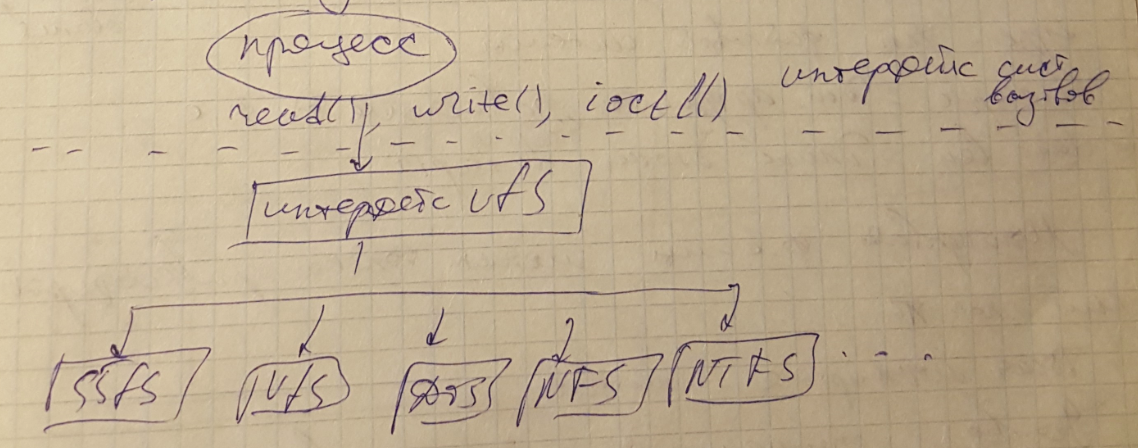
\includegraphics[width=\textwidth]{pic/1.png}
  \caption{Архитектура vfs}
\end{figure}

\begin{figure}[h!]
  \centering
  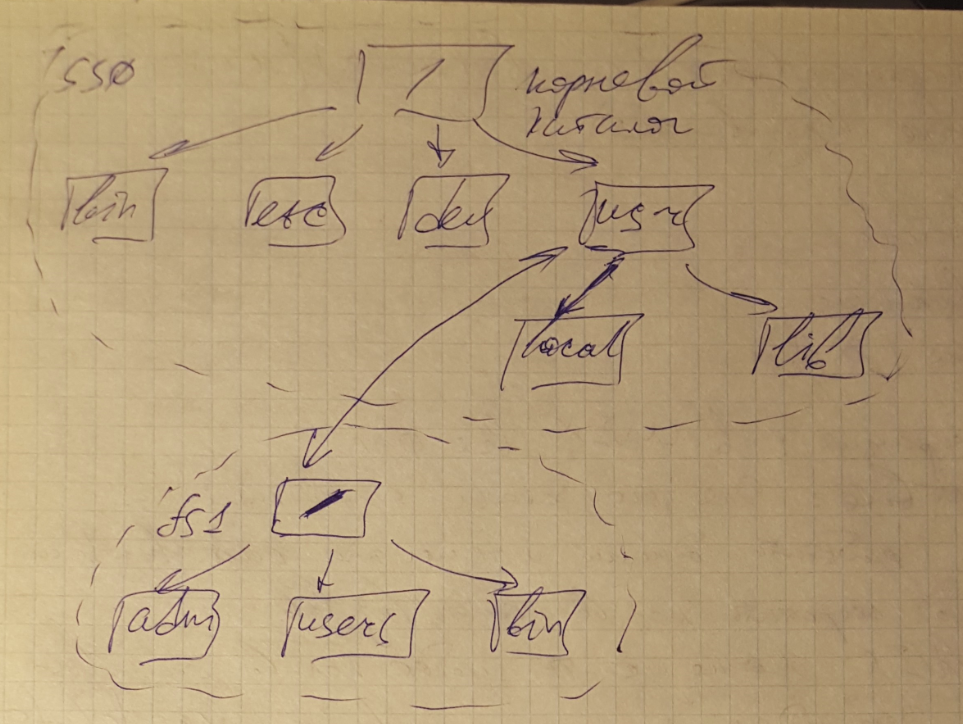
\includegraphics[width=\textwidth]{pic/2.png}
  \caption{pic}
\end{figure}

$/usr/lib$ – абсолютное имя. $./lib$ – относительное имя.

По \cite{UNIX_Internals} (стр 366):
$$mount (spec, dir, flags, type, dataptr, datalen);$$
$spec$ – имя файла – устройства, представляющего ФС;
$dir$ – полное имя каталога;
$type$ – тип файловой системы;
$dataptr$ – дополнительные аргументы, зависящие от ФС;
$datalen$ – длинна блока dataptr.

Монтировать ФС может только привилегированный пользователь.  Точка монтирования – каталог. Устройство – специальный файл, с помощью которого система получает доступ к физическому устройству. 

В командной строке функция монтирования выглядит так: 

$\# mount$ устройство точка\_монтирования

Даже ФС в разделе ЖД нужно монтировать. Отметим, что при инсталляции Linux и создании на ЖД раздела Linux, автоматически конфигурируется на монтировании основных ФС-м при каждом запуске.

$umount$ – команда, чтобы отмонтировать.

Файл – любая поименованная совокупность данных, размещенная на запоминающих устройствах.

Когда запускается процесс, он заинтересован в чтении/записи файлов. Библиотечные функции написаны для минимизации системных вызовов, т.к. системные вызовы переводят ОС в режим ядра.

Любой запущенные процесс имеет дескриптор в таблице процессов. Все открытые файлы описаны в таблице открытых файлов, которая одна на систему. (см. Рис. \ref{pic:proc_open_file})

\begin{figure}[H]
  \centering
  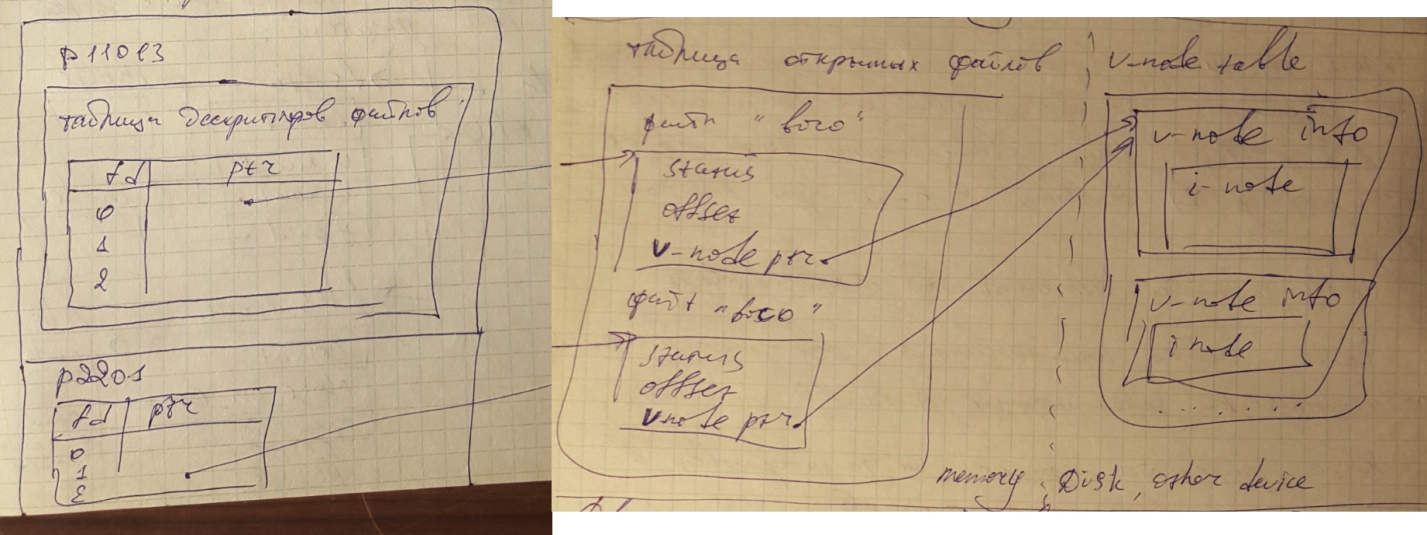
\includegraphics[width=\textwidth]{pic/3.png}
  \caption{pic}
  \label{pic:proc_open_file}
\end{figure}

На Рис. \ref{pic:proc_open_file} два процесса решили одновременно открыть один и тот же файл. Будет создано 2 дескриптора, описывающие открытый файл. В vnode ссылка на inode.

\begin{figure}[H]
  \centering
  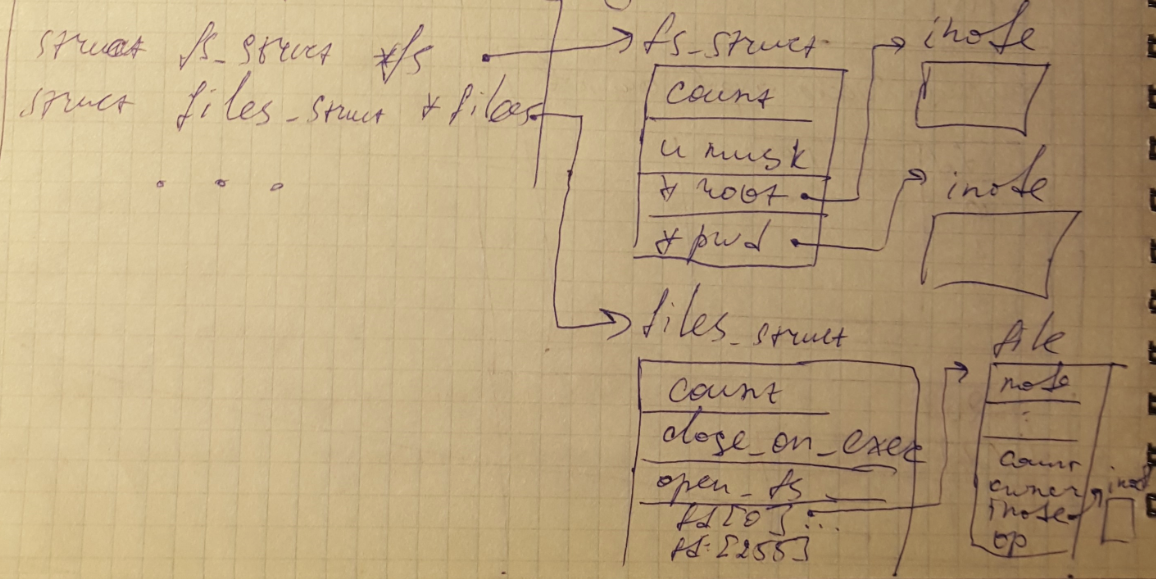
\includegraphics[width=\textwidth]{pic/4.png}
  \caption{pic}
  \label{pic:task_struct}
\end{figure}

$task\_struct$ – описывает процесс Linux. В ней есть указатели. (см. Рис. \ref{pic:task_struct})

\lstinputlisting[language=c, caption=Структура file]{listing/1.c} 


